% Section 8, Calibration.
\section{Calibration on Fresh Tasks}
\label{sec:calibration}

\subsection{The Label Run}
\label{sec:calib-labels}

\sysname's router assigns each incoming task to a fixer on the basis of per-task r\'{e}sum\'{e}s and cost thresholds (\S\ref{sec:system}).
Both mechanisms require outcome labels: which fixer solved which task, and at what price.
Public leaderboard data supplied these labels for several languages but contained zero usable Python outcomes for any fixer in the pool.
Benchmark contamination policies lock those results away, and Appendix~\ref{apx:bench-fresh} documents why leaderboard-derived labels mislead when applied outside their original distribution.
We therefore collected fresh labels: 100 Python bugs drawn from 2026 repositories, each attempted by all four fixers twice, once cold and once with \modelname's handoff injected (99 of the 100 yielded a valid paired comparison).
This paired design let every task serve as its own control, isolating the handoff's effect from task difficulty.

The same 100 tasks exposed a problem with \modelname's reproduction claims.
Replaying those claims against ground truth revealed that 32\% were genuine and 56\% demonstrably false.
The verify-then-strip gate described in \S\ref{sec:system} was built as a direct consequence, before any benchmark contact.

\subsection{The Handoff Redistributes}
\label{sec:calib-redist}

Figure~\ref{fig:redistribution} shows the paired comparison; exact rates and intervals appear in Appendix~\ref{apx:redistribution}.
Confidence intervals here and in the appendix are 95\% percentile
intervals from a bootstrap resampling tasks~\citep{bootstrap}.
The handoff lifted the three weaker fixers: \fxopus rose from 48.5\% to 53.5\% ($+5.1$\,pp, $p=0.125$), \fxkimi from 52.5\% to 56.6\% ($+4.0$\,pp, $p=0.481$), and \fxflash from 55.6\% to 57.6\% ($+2.0$\,pp,
$p=0.774$).
The strongest fixer, \fxgpt, moved in the opposite direction, dropping from 60.6\% to 56.6\% ($-4.0$\,pp, $p=0.424$).
Pooled across all four, the effect is $+1.8$ percentage points with a 95\% confidence interval of $[-1.0, {+}4.5]$ and $p=0.401$, not statistically significant.
At $N{=}99$ every per-fixer test is underpowered; the confidence intervals, not the point estimates, carry the information.

What the pattern does establish is that fixer rankings survive handoff conditioning, with only one adjacent flip falling within the confidence interval.
That stability is what the router's r\'{e}sum\'{e} assumption requires.
The pattern is consistent with redistribution rather than addition: solving ability shifts toward the cheaper models, which is exactly the shape cost-aware routing needs, though no single contrast reaches significance.
The redistribution pattern recurs on the benchmark's router-selected subset, though that comparison is uncontrolled and serves only as corroboration; exact numbers appear in Appendix~\ref{apx:pro-handoff}.

\begin{figure}[!tbp]
  \centering
  % ===========================================================================
% fig-redistribution.tex — paired solo -> with-handoff solve rate per fixer,
% label-run paired-100.
% BODY ONLY (tikzpicture). Wrapper/caption/label live in the section file.
% Requires % ===========================================================================
% fig-style.tex — shared colour / marker scheme for EVERY main-paper figure.
% \input this ONCE from the preamble of main.tex (after tikz + pgfplots).
%
% House rule: the palette is defined here and nowhere else. Each series also
% gets a distinct marker AND line style so the figures survive grayscale
% printing.
%
%   \sysname / deployed .. cSys   (blue!70!black)    mark *
%   opus / claude ........ cOpus  (red!70!black)     mark square*
%   gpt .................. cGpt   (teal!70!black)    mark triangle*
%   kimi ................. cKimi  (violet!70!black)  mark diamond*
%   flash ................ cFlash (orange!70!black)  mark pentagon*
%   greedy / baseline .... cBase  (gray)             mark o
% ===========================================================================
% The pipeline diagram needs the calc library for coordinate arithmetic; the
% rest of the libraries are already loaded in main.tex's preamble.
\usetikzlibrary{calc}
% Hatching, so bar charts stay readable in grayscale.
\usetikzlibrary{patterns}

\colorlet{cSys}{blue!70!black}
\colorlet{cOpus}{red!70!black}
\colorlet{cGpt}{teal!70!black}
\colorlet{cKimi}{violet!70!black}
\colorlet{cFlash}{orange!70!black}
\colorlet{cBase}{gray}

% Common axis furniture: footnotesize ticks/legend, small titles, framed
% legend in gray!50, light horizontal grid.
\pgfplotsset{
  paperaxis/.style={
    width=0.80\linewidth,
    height=5.2cm,
    tick label style={font=\footnotesize},
    label style={font=\footnotesize},
    title style={font=\small},
    legend style={font=\footnotesize, draw=gray!50, fill=white,
                  fill opacity=0.9, text opacity=1, rounded corners=1pt},
    every axis plot/.append style={line width=0.7pt},
    grid style={gray!25, line width=0.3pt},
    axis line style={gray!60},
    tick style={gray!60},
  },
  papermark/.style={mark size=2.6pt},
}
 in the preamble.
%
% PROVENANCE — every number.
%   Source: internal records, the DIRECTIONAL-ONLY handoff section, the paired
%   table (N=99 paired tasks, same task / same fixer, Delta = handoff - solo):
%
%     fixer    solo    handoff   Delta pp (95% CI)      McNemar p
%     claude   48.5    53.5      +5.1  [ 0.0, 10.1]     0.125
%     kimi     52.5    56.6      +4.0  [-4.0, 12.1]     0.481
%     flash    55.6    57.6      +2.0  [-5.1,  9.1]     0.774
%     gpt      60.6    56.6      -4.0  [-11.1, 3.0]     0.424
%     pooled   54.3    56.1      +1.8  [-1.0,  4.5]     0.401
%
%   Absolute solo and handoff rates ARE present in that table, so nothing is
%   derived here beyond one addition, stated explicitly:
%   THE PLOTTED INTERVAL is the published paired-DELTA CI anchored at the
%   published solo rate, i.e. [solo + CI_low, solo + CI_high]:
%     claude  [48.5, 58.6]   kimi  [48.5, 64.6]   flash [50.5, 64.7]
%     gpt     [49.5, 63.6]   pooled[53.3, 58.8]
%   The source reports NO CI on the absolute rates themselves; the interval
%   must therefore always be described as a delta CI, never as a CI on the
%   handoff rate. No other arithmetic was performed.
%
%   Scope stamp (binding, from the same file's header): N=99 paired / 100
%   solo, Python-only, label run. "N=99-100 underpowers every per-fixer
%   significance test — read the CIs, not the point estimates." No fixer
%   reaches p<0.05; every effect is DIRECTIONAL-ONLY.
% ===========================================================================
\begin{tikzpicture}
\begin{axis}[
  paperaxis,
  width=0.80\linewidth,
  height=5.2cm,
  xmin=44, xmax=70,
  xtick={45,50,55,60,65},
  xticklabel={\pgfmathprintnumber{\tick}\%},
  xlabel={Solve rate (paired, $N{=}99$)},
  symbolic y coords={{claude},{kimi},{flash},{gpt},{pooled}},
  ytick=data,
  % internal symbolic-coordinate keys above stay bare identifiers for
  % pgfplots bookkeeping; the RENDERED tick labels go through the fixer
  % macros so no bare family name ever reaches the page.
  yticklabels={\fxopus,\fxkimi,\fxflash,\fxgpt,pooled},
  y dir=reverse,
  enlarge y limits=0.16,
  xmajorgrids=true,
  legend style={at={(0.5,-0.26)}, anchor=north, legend columns=2,
                /tikz/every even column/.append style={column sep=6pt}},
  legend cell align=left,
]

% ---- paired-delta 95% CI, anchored at the solo rate --------------------
% [solo + CI_low, solo + CI_high]; see the provenance block above.
\draw[gray!45, line width=0.6pt] (axis cs:48.5,{claude}) -- (axis cs:58.6,{claude});
\draw[gray!45, line width=0.6pt] (axis cs:48.5,{kimi})   -- (axis cs:64.6,{kimi});
\draw[gray!45, line width=0.6pt] (axis cs:50.5,{flash})  -- (axis cs:64.7,{flash});
\draw[gray!45, line width=0.6pt] (axis cs:49.5,{gpt})    -- (axis cs:63.6,{gpt});
\draw[gray!45, line width=0.6pt] (axis cs:53.3,{pooled}) -- (axis cs:58.8,{pooled});
% end caps
\draw[gray!45, line width=0.6pt] ([yshift=2.2pt] axis cs:48.5,{claude}) -- ([yshift=-2.2pt] axis cs:48.5,{claude});
\draw[gray!45, line width=0.6pt] ([yshift=2.2pt] axis cs:58.6,{claude}) -- ([yshift=-2.2pt] axis cs:58.6,{claude});
\draw[gray!45, line width=0.6pt] ([yshift=2.2pt] axis cs:48.5,{kimi})   -- ([yshift=-2.2pt] axis cs:48.5,{kimi});
\draw[gray!45, line width=0.6pt] ([yshift=2.2pt] axis cs:64.6,{kimi})   -- ([yshift=-2.2pt] axis cs:64.6,{kimi});
\draw[gray!45, line width=0.6pt] ([yshift=2.2pt] axis cs:50.5,{flash})  -- ([yshift=-2.2pt] axis cs:50.5,{flash});
\draw[gray!45, line width=0.6pt] ([yshift=2.2pt] axis cs:64.7,{flash})  -- ([yshift=-2.2pt] axis cs:64.7,{flash});
\draw[gray!45, line width=0.6pt] ([yshift=2.2pt] axis cs:49.5,{gpt})    -- ([yshift=-2.2pt] axis cs:49.5,{gpt});
\draw[gray!45, line width=0.6pt] ([yshift=2.2pt] axis cs:63.6,{gpt})    -- ([yshift=-2.2pt] axis cs:63.6,{gpt});
\draw[gray!45, line width=0.6pt] ([yshift=2.2pt] axis cs:53.3,{pooled}) -- ([yshift=-2.2pt] axis cs:53.3,{pooled});
\draw[gray!45, line width=0.6pt] ([yshift=2.2pt] axis cs:58.8,{pooled}) -- ([yshift=-2.2pt] axis cs:58.8,{pooled});

% ---- solo -> handoff connectors ---------------------------------------
\draw[-{Stealth[length=2.0mm]}, black!65, line width=0.7pt] (axis cs:48.5,{claude}) -- (axis cs:53.5,{claude});
\draw[-{Stealth[length=2.0mm]}, black!65, line width=0.7pt] (axis cs:52.5,{kimi})   -- (axis cs:56.6,{kimi});
\draw[-{Stealth[length=2.0mm]}, black!65, line width=0.7pt] (axis cs:55.6,{flash})  -- (axis cs:57.6,{flash});
\draw[-{Stealth[length=2.0mm]}, black!65, line width=0.7pt] (axis cs:60.6,{gpt})    -- (axis cs:56.6,{gpt});
\draw[-{Stealth[length=2.0mm]}, black!65, line width=0.7pt] (axis cs:54.3,{pooled}) -- (axis cs:56.1,{pooled});

% ---- solo (open, gray) -------------------------------------------------
\addplot[only marks, papermark, color=cBase, mark=o, mark options={fill=white}]
  coordinates {(48.5,{claude}) (52.5,{kimi}) (55.6,{flash})
               (60.6,{gpt}) (54.3,{pooled})};
\addlegendentry{solo}

% ---- with handoff (filled, per-fixer colour + distinct marker) ---------
\addplot[only marks, papermark, color=cOpus, mark=square*]
  coordinates {(53.5,{claude})};
\addlegendentry{with handoff}
\addplot[only marks, papermark, color=cKimi, mark=diamond*, forget plot]
  coordinates {(56.6,{kimi})};
\addplot[only marks, papermark, color=cFlash, mark=pentagon*, forget plot]
  coordinates {(57.6,{flash})};
\addplot[only marks, papermark, color=cGpt, mark=triangle*, forget plot]
  coordinates {(56.6,{gpt})};
\addplot[only marks, papermark, color=cSys, mark=*, forget plot]
  coordinates {(56.1,{pooled})};

% ---- delta labels ------------------------------------------------------
\node[font=\scriptsize, text=cOpus,  anchor=west] at (axis cs:59.2,{claude}) {$+5.1$};
\node[font=\scriptsize, text=cKimi,  anchor=west] at (axis cs:65.2,{kimi})   {$+4.0$};
\node[font=\scriptsize, text=cFlash, anchor=west] at (axis cs:65.3,{flash})  {$+2.0$};
\node[font=\scriptsize, text=cGpt,   anchor=west] at (axis cs:64.2,{gpt})    {$-4.0$};
\node[font=\scriptsize, text=cSys,   anchor=west] at (axis cs:59.4,{pooled}) {$+1.8$};

\end{axis}
\end{tikzpicture}

  \caption{\textbf{The handoff pattern is redistributive, not additive.}
  Paired comparison ($N{=}99$ tasks, four fixers).  Open circles: solo
  rates; filled markers: with-handoff.  Horizontal bars span the 95\%
  CI of each paired delta, anchored at the solo rate.  The three weaker
  fixers gain; the strongest loses.  All deltas are directional only
  ($p>0.05$ at this sample size).}
  \label{fig:redistribution}
\end{figure}

\subsection{The Router Design Space}
\label{sec:calib-design}

We compared four input-feature variants under an offline simulation of the capped cost protocol, pinning each to the same matched solve rate so that the bars in Figure~\ref{fig:design-space} differ only in spend.
Variant~A, using task text alone, saves 30.5\% on total cost per solve at a matched solve rate.
Adding \modelname's hidden states produces variant~C, the routing blend, raising the saving to 34.3\%.
The two variants that incorporate handoff-text features tell a sharply different story: variant~B collapses to 8.0\% and variant~D to 9.4\%.
The lesson is concrete.
The searcher's internal state helps the router, while the handoff's text helps the fixers; feeding the handoff memo to the router actively hurts.

Supporting signals reinforce this split.
As an outcome predictor, the hidden state reaches an AUC of 0.600 (fold-stable in four of five folds), while handoff text manages only 0.510.
A simple logistic regression beat a multi-layer perceptron in every comparison, so the simpler scorer shipped.
The full grid appears in Appendix~\ref{apx:design-space}.
The C-versus-A cost gap, a different quantity from the AUC separation,
holds in only three of five folds, and the gate-level caveat of \S\ref{sec:results} applies: at deployment the hidden state's informational contribution cannot be fully separated from its threshold-shifting effect.
On the calibration labels, the cost-aware router matched the strongest fixer's solve rate at 29\% lower total cost per solve (\$0.49 versus \$0.69).

\begin{figure}[!tbp]
  \centering
  % ===========================================================================
% fig-design-space.tex — router input design space: held-out cost saving by
% feature variant.
% BODY ONLY (tikzpicture). Wrapper/caption/label live in the section file.
% Requires % ===========================================================================
% fig-style.tex — shared colour / marker scheme for EVERY main-paper figure.
% \input this ONCE from the preamble of main.tex (after tikz + pgfplots).
%
% House rule: the palette is defined here and nowhere else. Each series also
% gets a distinct marker AND line style so the figures survive grayscale
% printing.
%
%   \sysname / deployed .. cSys   (blue!70!black)    mark *
%   opus / claude ........ cOpus  (red!70!black)     mark square*
%   gpt .................. cGpt   (teal!70!black)    mark triangle*
%   kimi ................. cKimi  (violet!70!black)  mark diamond*
%   flash ................ cFlash (orange!70!black)  mark pentagon*
%   greedy / baseline .... cBase  (gray)             mark o
% ===========================================================================
% The pipeline diagram needs the calc library for coordinate arithmetic; the
% rest of the libraries are already loaded in main.tex's preamble.
\usetikzlibrary{calc}
% Hatching, so bar charts stay readable in grayscale.
\usetikzlibrary{patterns}

\colorlet{cSys}{blue!70!black}
\colorlet{cOpus}{red!70!black}
\colorlet{cGpt}{teal!70!black}
\colorlet{cKimi}{violet!70!black}
\colorlet{cFlash}{orange!70!black}
\colorlet{cBase}{gray}

% Common axis furniture: footnotesize ticks/legend, small titles, framed
% legend in gray!50, light horizontal grid.
\pgfplotsset{
  paperaxis/.style={
    width=0.80\linewidth,
    height=5.2cm,
    tick label style={font=\footnotesize},
    label style={font=\footnotesize},
    title style={font=\small},
    legend style={font=\footnotesize, draw=gray!50, fill=white,
                  fill opacity=0.9, text opacity=1, rounded corners=1pt},
    every axis plot/.append style={line width=0.7pt},
    grid style={gray!25, line width=0.3pt},
    axis line style={gray!60},
    tick style={gray!60},
  },
  papermark/.style={mark size=2.6pt},
}
 in the preamble.
%
% PROVENANCE — every number.
%   Primary source: internal records, the definitive 4-row comparison on the
%   combined deployable router, column "saving %" (all four rows at the SAME matched accuracy .606,
%   fold-held-out, N=99, anchor = always-best gpt at $0.406 / .606):
%     A  task text only                              +30.5%  ($0.2824/task)
%     B  task text + handoff text                    + 8.0%  ($0.3734/task)
%     C  task text + hidden states                   +34.3%  ($0.2668/task)
%     D  task text + handoff text + hidden states    + 9.4%  ($0.3677/task)
%   Cross-checked against the same source's head-ablation table (LR rows:
%   30.5 / 8.0 / 34.3 / 9.4 — identical). Variant C, the text+hidden-state
%   blend, is the router's head; variant A is the text-only comparison.
%   The "handoff-text features hurt cost routing" reading is the source's
%   own: "The handoff-text embedding is a bad blend partner: averaging it in
%   (variants B and D) drags the saving down to ~8-9% ... so more features is
%   not better, the right feature is."
%   Fold stability (context, not plotted): A 3/5, B 1/5, C 3/5, D 4/5 vs
%   anchor; variant C's ~4pp gain over A is explicitly "not bankable at
%   N=99".
% ===========================================================================
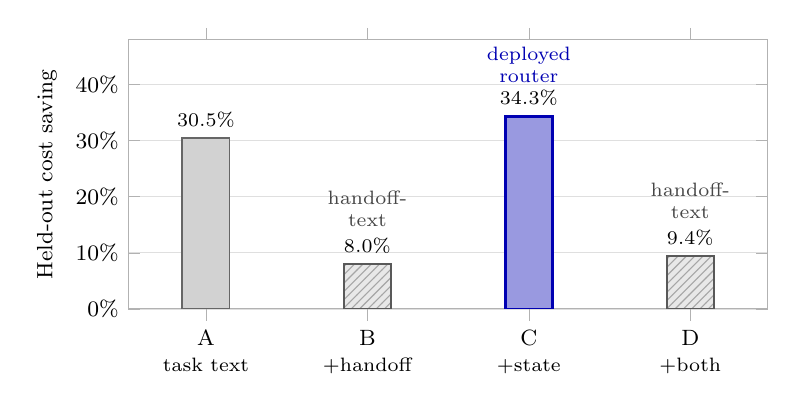
\begin{tikzpicture}
\begin{axis}[
  paperaxis,
  width=0.80\linewidth,
  height=5.0cm,
  ybar,
  bar width=17pt,
  ymin=0, ymax=48,
  ytick={0,10,20,30,40},
  yticklabel={\pgfmathprintnumber{\tick}\%},
  ylabel={Held-out cost saving},
  symbolic x coords={{A},{B},{C},{D}},
  xtick={{A},{B},{C},{D}},
  xticklabels={A\\{\scriptsize task text}, B\\{\scriptsize $+$handoff},
               C\\{\scriptsize $+$state}, D\\{\scriptsize $+$both}},
  xticklabel style={font=\footnotesize, align=center},
  enlarge x limits=0.16,
  ymajorgrids=true,
  nodes near coords={\pgfmathprintnumber[fixed, fixed zerofill, precision=1]{\pgfplotspointmeta}\%},
  nodes near coords style={font=\scriptsize},
]

% ---- A: text-only baseline --------------------------------------------
\addplot[fill=cBase!35, draw=cBase!80!black, bar shift=0pt]
  coordinates {({A},30.5)};

% ---- B and D: variants carrying handoff-text features (hatched) --------
\addplot[fill=cBase!18, draw=cBase!70!black, bar shift=0pt,
         postaction={pattern=north east lines, pattern color=cBase!70}]
  coordinates {({B},8.0) ({D},9.4)};

% ---- C: the winner, the deployed router --------------------------------
\addplot[fill=cSys!40, draw=cSys, line width=1.0pt, bar shift=0pt]
  coordinates {({C},34.3)};

% ---- winner callout ----------------------------------------------------
\node[font=\scriptsize, text=cSys, anchor=south, align=center]
  at (axis cs:{C},38.6) {deployed\\router};

% ---- the two handoff-text variants -------------------------------------
\node[font=\scriptsize, text=gray!55!black, anchor=south, align=center]
  at (axis cs:{B},13.0) {handoff-\\text};
\node[font=\scriptsize, text=gray!55!black, anchor=south, align=center]
  at (axis cs:{D},14.4) {handoff-\\text};

\end{axis}
\end{tikzpicture}

  \caption{\textbf{Which router features buy cost savings.}
  Held-out cost saving against an always-best-model anchor, all variants
  pinned to the same solve rate ($.606$).  Adding \modelname's hidden
  states (variant~C, the routing blend) lifts savings from $30.5\%$ to $34.3\%$.
  Variants with handoff-text features (B,~D) collapse to $8$--$9\%$.
  The C-vs-A gap is fold-fragile at $N{=}99$.}
  \label{fig:design-space}
\end{figure}

Calibration settled four design choices: the routing blend (variant~C), the matched-point threshold ($\theta{=}0.30$), logistic regression as the scoring function, and blanket handoff injection.
It left one question open.
\fxgpt was the strongest fixer on these fresh tasks, a ranking the benchmark later inverted (\S\ref{sec:results}).

\FloatBarrier
